\documentclass[border=6pt]{standalone}
\usepackage[T1]{fontenc}\usepackage{lmodern}\usepackage{amsmath,amssymb}\usepackage{graphicx}\usepackage{xcolor}\usepackage{tikz}
\usetikzlibrary{arrows.meta,positioning,calc,fit,shapes.misc,shapes.geometric}
% TikZ styles
\tikzset{
  blk/.style={draw, rounded corners=2pt, align=center, font=\small, minimum height=8mm, inner sep=4pt, fill=#1},
  blk/.default=white,
  arr/.style={-{Stealth[length=2.2mm]}, thick},
}
\definecolor{base}{HTML}{FBE3E3}
\definecolor{prop}{HTML}{DDEBFA}
\definecolor{same}{HTML}{EDEDED}
\definecolor{done}{HTML}{DFF1DF}
\definecolor{todo}{HTML}{FFF2CC}

\begin{document}
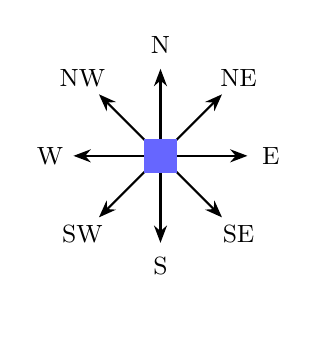
\begin{tikzpicture}[scale=0.85, baseline={(0,-2.2)}]
    \foreach \a/\l in {90/N,270/S,0/E,180/W,45/NE,135/NW,315/SE,225/SW}{
      \draw[arr] (0,0) -- (\a:1.3);
      \node[font=\small] at (\a:1.65) {\l};}
    \fill[blue!60] (-0.25,-0.25) rectangle (0.25,0.25);
  \end{tikzpicture}
\end{document}
